\documentclass[12pt]{article}
\usepackage{fontspec}
\setmainfont{Arial}
\usepackage{wrapfig}
\usepackage[english]{babel}

\usepackage{setspace}
\singlespacing

% normal box
\newcommand{\sqboxs}{1.2ex}% the square size
\newcommand{\sqboxf}{0.6pt}% the border in \sqboxEmpty
\newcommand{\sqbox}[1]{\textcolor{#1}{\rule{\sqboxs}{\sqboxs}}}

%\usepackage[none]{hyphenat}
%\usepackage{hyphenat}

\usepackage{graphicx}
\usepackage{caption}
%\usepackage[T1]{fontenc}
%\usepackage[utf8]{inputenc}
\usepackage{lmodern}
\usepackage{geometry}
\geometry{
	a4paper,
	left=20mm,
	right=20mm,
	top=25mm,
	bottom=25mm,
}

\usepackage{pgfgantt}
\usepackage{eurosym}

\usepackage{pdfpages}


\usepackage{subcaption}

\usepackage[unicode=true,pdfusetitle,bookmarks=true,bookmarksnumbered=false,bookmarksopen=false,
breaklinks=false,pdfborder={0 0 0},backref=false,colorlinks=true,urlcolor=magenta]{hyperref}

\usepackage{multibib}
\newcites{article,conf,confnoproc}{{Articles dans des revues internationales à comité de lecture
	},{Communications dans des congrès internationaux à comité de lecture et actes
		publiés},{Communications dans des congrès internationaux sans comité de lecture}}


\newcommand{\review}[1]{\textcolor{blue}{#1}}

\graphicspath{{images/}}

\author{Andrea Brugnoli \\ 
	\hspace{2.8pt} PhD ISAE-SUPAERO 2020\\
	Msc ISAE-SUPAERO 2017}
\title{Research project}

\date{}

\begin{document}
	
	\maketitle
	
	\tableofcontents

	
	
	\section{The big picture}
	
	The goal of my research project is to implement numerical methods to accelerate the simulation of
	to accelerate the simulation of fluid-structure interaction (FSI) problems, compared to the computational time required for a high-fidelity simulation. This will make it possible to integrate more economical models, which can replace very expensive simulations. This will also facilitate optimized system component design and decision making. Unlike many methods proposed in the literature, the imperative is fidelity to the physical structure of the problem.  This structure is most often ignored by reduction algorithms, which treat simulations as black boxes. Physically faithful reduced models are much more accurate than nonphysical ones, and their use can radically improve the techniques normally used for optimization. To achieve its ambition, this project aims at using recent mathematical formalisms for multiphysics modeling and model digitization.
	
	
	\section{Development of the scientific project}
	
	\subsection{Multiphysics problems}
	Computational engineering is a recent, multidisciplinary and rapidly expanding science. Its goal is to implement mathematical and numerical models to predict the behavior of complex systems. This allows to design ex novo systems or to detect faults during the life cycle of components, without having to use very expensive experimental tests. This field is rapidly expanding because today we have more powerful computers and especially because the algorithms have been optimized to be faster, more robust and easier to use. However, multiphysics problems, which are central to industrial applications, are extremely complicated to handle. This is due on the one hand to the difficulty associated with the treatment of the different physics and on the other hand to the size of the resulting systems, which require several days, or even weeks, to be solved using a supercomputer \cite{keyes2013}. These problems pose barriers for the use of numerical models in industry. 
	
	
	\subsection{Scientific tools of the project}
	
	\paragraph{A unifying formalism for the modelisation of dynamical systems : port-Hamiltonian system theory\\}

	
	A very promising mathematical formalism for dealing with multiphysics problems is the port-Hamiltonian formalism \cite{vanderSchaft2002}, based on Hamiltonian mechanics and bond graphs modeling. At the heart of this formalism, there is the idea that any physical system can be described in a modular way. Simple components interact with each other and with the surrounding environment through ports. The interaction ports contain information about the flow of energy between the different components and between different physical domains, e.g. mechanical, electromagnetic, thermal. Modular design is central to engineering, as the design of any technological system is made from simple elements that are assembled to give rise to the complexity that surrounds us. Take for example an airplane, a helicopter, a satellite (cf. Fig. \ref{fig:satellite}): to be able to optimize their design it is essential to have a modeling tool able to decompose the complexity in order to find the different key components. The use of a unified modeling tool will allow the creation of a common infrastructure for the digital implementation in an industrial context.



	\begin{figure}[hb]
		\centering
		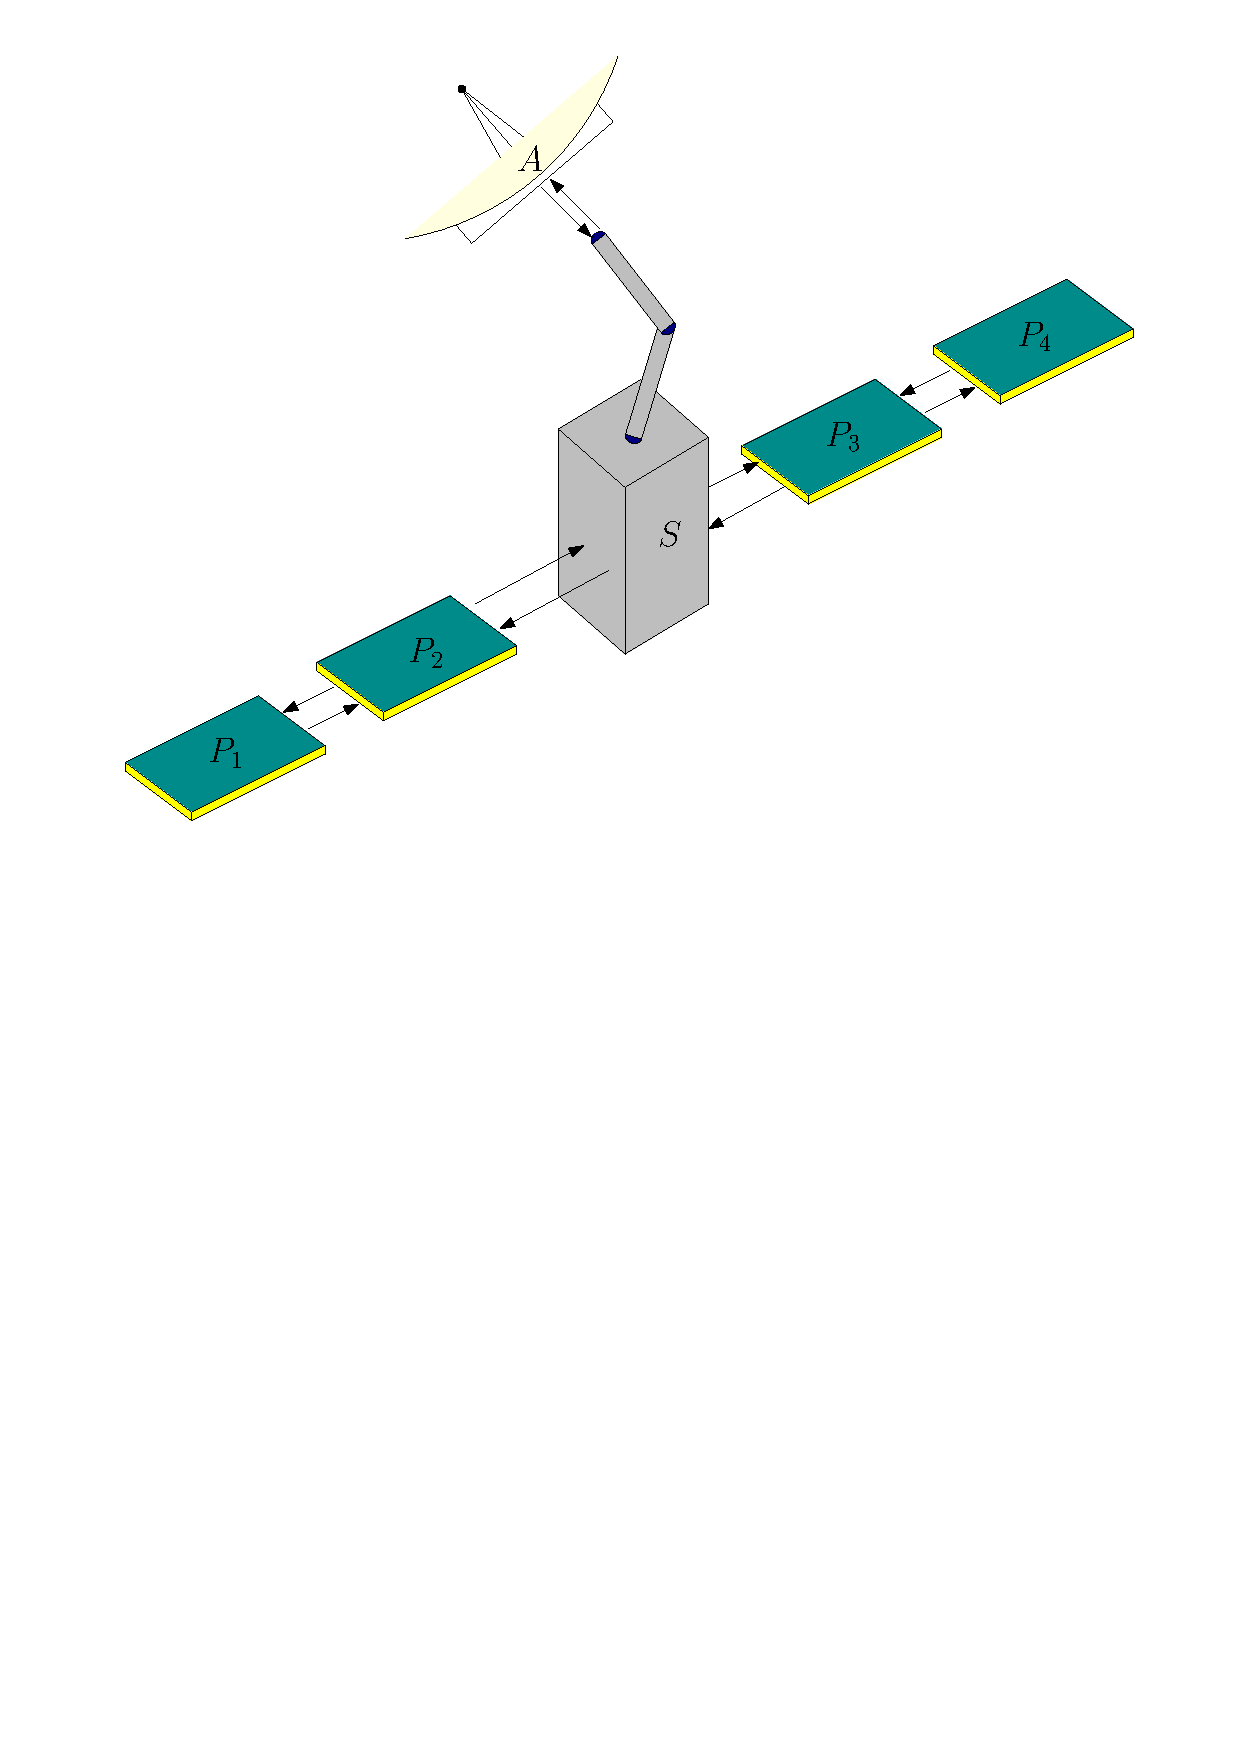
\includegraphics[width=.55\textwidth]{satellite.pdf}
		\caption{Schéma modulaire représentant un satellite de télécommunication.}
		\label{fig:satellite}
	\end{figure}
	
	\paragraph{A structured methodology for discretization\\}
	
	The numerical algorithms used in industry are adapted to the physical nature of the problem. For solid mechanics, the finite element method is the de facto standard. For fluid dynamics, finite volumes are mostly used because they guarantee the fulfillment of conservation laws. When these two approaches must be used simultaneously, their coupling poses several challenges. The two methods use different degrees of freedom (i.e. different topological entities of the mesh) and the interconnection inevitably introduces errors. A general modeling tool requires an equally general discretization method, able to guarantee the possibility of interconnecting distinct physics. Recently, a unifying formalism for the discretization of partial differential equations has been developed \cite{arnold2006acta}. This mathematical theory, called finite element method exterior calculus or FEEC\footnote{Exterior calculus is a generalization of vector calculus based on differential geometry}, has allowed important developments for the discretization of partial differential equations from physics. It has been successfully applied to solid mechanics, fluid dynamics and electromagnetism and represents a powerful tool for multiphysics applications. The significance of this theory is illustrated by the fact that the United Kingdom has decided to renew the codes for meteorology using a FEEC based computational core\footnote{The site \url{https://www.metoffice.gov.uk/research/news/2021/gungho-and-lfric-10th-anniversary} gives an overview of the project. The interested reader can also consult the slides  \url{https://www.ecmwf.int/sites/default/files/elibrary/2016/16815-introduction-lfric-project.pdf}}.
	
	\paragraph{Artificial intelligence for model order reduction\\}
	Any discretization method, even the most sophisticated, leads to systems whose size easily exceeds one million unknowns. In order to optimize the design of mechanical components, these models must be simulated several times. This leads to prohibitive computational costs even for companies with the most advanced computing centers. It is therefore essential to introduce reduction methods, which are supposed to build a simpler model, capable of retaining the main properties of the original system. The vast majority of these methods assume that one can obtain a reduced system through an essentially linear method, i.e. the Orthogonal Decomposition into Eigenvalues (ODE). This assumption is not valid for any system exhibiting a nonlinear behavior and leads to overestimate the dimension of the reduced system. Thanks to recent progress in the field of Artificial Intelligence (AI), new methods allow to obtain more efficient reduced models. For example, researchers have proposed an architecture based on convolutional neural networks to obtain much faster models (by a factor of about 100) compared to high fidelity discretizations. Their technique represents a non-linear extension of commonly used methodologies. The results obtained demonstrate the performance gain that can be obtained by using convolutional neural networks (see Fig. \ref{fig:deepROM}).
	
	\begin{figure}[t]
		\begin{subfigure}[t]{0.465\textwidth}
			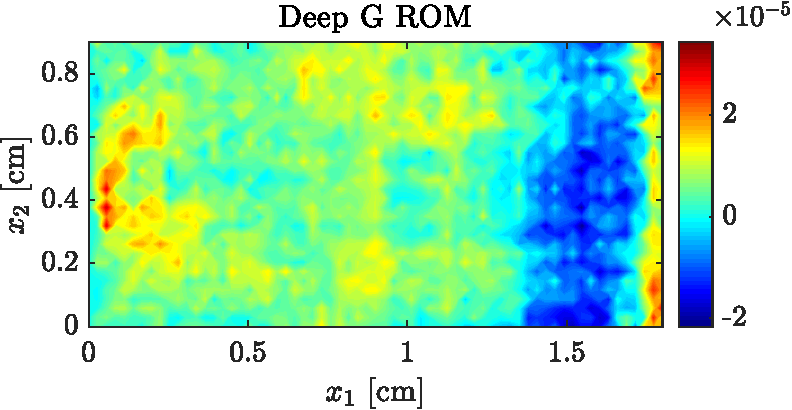
\includegraphics[width=\columnwidth]{DGROM_T_param1.pdf} 
			\caption{Convolutional neural networks based MOR.}
			\label{fig:DG_ROM}
		\end{subfigure}\hfill
		\begin{subfigure}[t]{0.48\textwidth}
			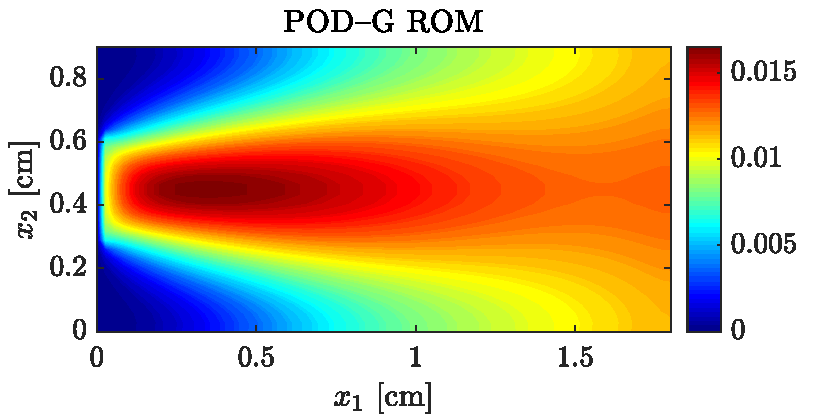
\includegraphics[width=\columnwidth]{GROM_T_param1.pdf}%
			\caption{POD based MOR}
			\label{fig:POD_ROM}
		\end{subfigure}
		\caption[]{Error of reduced models on the temperature field for a convection-diffusion-reaction problem. By using a convolutional neural network to generate a nonlinear variety (see Fig. \ref{fig:DG_ROM}) the error associated with the reduction is drastically reduced, from $10^{-2}$ to $10^{-5}$, compared to the POD method (see Fig. \ref{fig:POD_ROM}). Reproduced from \cite{lee2020} with permission.}%
		\label{fig:deepROM}%
	\end{figure}
	
	
	\subsection{Scientific challenges and work packages}
	The first challenge is related to the resolution of coupled multiphysics systems.  In the industry different methods are usually used to simulate different physics. Therefore, it is often necessary to integrate different solvers and software to simulate these problems. This leads to an increase in the complexity of industrial procedures. Moreover, the numerical coupling does not represent correctly the energy flows. \\
	
	The first work package (\textbf{WP1}) seeks to solve the problems related to the multiphysics coupling, in a way to guarantee the respect of energy flows between different physics. These numerical models will have to retain the physical properties of the problem (global energy conservation, tracing of energy exchanges between the different subsystems, invariants of the problem). \\
	
	\begin{itemize}
		\item \textbf{WP1} : Development of high-fidelity numerical algorithms for fluid-structure interaction problems, based on the finite element in external calculation and the port-Hamiltonian formalism. \\
	\end{itemize}
	
	The use of a unified modeling paradigm will allow the couplings to be performed in a physics-compliant manner.
	
	The second scientific lock concerns the integration of techniques from AI to obtain physical reduced models. This is a recent but rapidly expanding research theme. For the moment, artificial intelligence is mainly used to automate simple tasks, such as the automatic classification of images, text, videos, etc. Despite the recent achievements of algorithms capable of outperforming humans in board games such as chess or go, the use of AI for computational physics is still in an embryonic state. It is extremely important to understand the advantages and limitations of these techniques in order to integrate them into the set of numerical tools that have already proven themselves in physical modeling. \\
	
	The second work package (WP2) aims at generating reduced models able to incorporate the physics of the problem in an interpretable way. \\
	
	\begin{itemize}
		\item \textbf{WP2} : Reduction methods guaranteeing the respect of the physical structure implemented using neural networks.
	\end{itemize}
	
	This work package will allow to obtain small dimensional models, ready to be used for the optimization part. 
	
	Optimization and parametric studies are typically performed on substitution models in industry
	Optimization and parametric studies are typically performed on surrogate models in industry, because optimizing fine models directly involves absolutely prohibitive computational costs. It is very difficult to know in advance which method to use to generate a surrogate model for a certain physical problem. The reliability of these models is also difficult to predict, since the physical meaning is destroyed by the reduction procedure. \\
	
	The final objective of the project is to demonstrate that the reduced models obtained in the \textbf{WP2} will be able to serve as more reliable surrogate models than those normally used. In the third work package (WP3) the reduced models will be used to optimize the mechanical design of structures and for the optimal control of flexible structures. This step will allow to evaluate the validity and efficiency of the reduced models compared to the fine simulations. \\
	
	\begin{itemize}
		\item \textbf{WP3} : Use of reduced models for optimization and optimal control and comparison with high-fidelity models. \\
	\end{itemize}
	
	Solving these three macro-tasks will provide a better understanding of the trade-off between computational time and accuracy for applications of industrial interest. Potentially, the techniques developed in this project will provide solutions that are more efficient than those normally used in industry. 
	
	
	\bibliographystyle{unsrt}
	\bibliography{biblio_recherche}
	
	
\end{document}
